% This is main.tex, a sample paper demonstrating the use of the
% LLNCS macro package for Springer Computer Science proceedings;
% Version 2.20 of 2017/10/04
% 
\documentclass[runningheads]{llncs}
\usepackage[a4paper,left=3cm,right=3cm,top=4cm,bottom=4cm,bindingoffset=5mm]{geometry}
%
% ---- Packages ----
%
\usepackage{graphicx} % enhanced support for graphics
\usepackage{subcaption}
\usepackage{url} % add macros for handling URLs in text
\usepackage[nohyperlinks,nolist]{acronym} % abbreviation utilities
\usepackage{listings}
\usepackage{svg}
% TODO: add more packages below if necessary
%
% ---- Acronyms ----
%
\begin{acronym}
\acro{rq}[RQ]{Research Question}
\acro{llm}[LLM]{Large Language Model}
\acro{html}[HTML]{Hypertext Markup Language}
\acro{nlp}[NLP]{natural language processing}
\acro{dom}[DOM]{Document Object Model}
\acro{rted}[RTED]{Robust Tree Edit Distance}
\acro{rnn}[RNN]{Recurring Neural Network}
\acro{lstm}[LSTM]{Long Short-Term Memory}
\acro{apted}[APTED]{All Path Tree Edit Distance}
\acro{vips}[VIPS]{Vision-based Page Segmentation}
% TODO: define more acronyms here
\end{acronym}
%
% ---- 
%
% ---- Begin Document ----
%
\begin{document}
%
\title{Similarity Classification of HTML with Large Language Models}
%
%\titlerunning{Abbreviated paper title}
% If the paper title is too long for the running head, you can set
% an abbreviated paper title here
%
% ---- Author Information ----
%
\author{Timo Kühne}
\institute{Seminar: Software Quality\\
Advisor: Andrea Stocco\\
Technical University of Munich\\
\email{timo.kuehne@tum.de}}
%
\maketitle % typeset the header of the contribution
%
% ---- Abstract ----
%
\begin{abstract}
    
\begin{itemize}
    Web application testing is crucial to ensure software quality and reliability. Successful test automation reduces the need for manual testing. However, near-duplicate web pages, i.e. different pages with the overall same functionality, pose a significant challenge for effective test automation. Detecting these near-duplicates is essential for creating efficient test suites that avoid redundant test cases while maintaining comprehensive coverage. This paper presents GeminiScan, a novel approach leveraging \acp{llm} for near-duplicate detection in web testing. Our method combines a small-scale \ac{llm} for efficient inference with a large-scale \ac{llm} for prompt optimization, addressing the limitations of existing techniques in semantic understanding and generalization.
    We evaluate GeminiScan on a subset of the widely-used Yandrapally et al. 2020 dataset, focusing on two web applications: Addressbook (PHP-based) and PetClinic (JavaScript-based). Our approach achieves F1 scores of 0.87 and 0.78 for Addressbook and PetClinic, respectively outperforming traditional methods like RTED and approaching the performance of state-of-the-art techniques such as WebEmbed and FragGen.
    GeminiScan performs well in identifying distinct pages and effectively detects near-duplicates, with an average classification time of 455ms for Addressbook and 350ms for PetClinic on an Nvidia A100 GPU. Our method shows particular strength in avoiding false positives, rarely misclassifying near-duplicates as distinct.
    This research contributes to the field by demonstrating the potential of \acp{llm} in web testing, offering a generalizable approach that balances efficiency and effectiveness. While computational requirements present a current challenge, the rapid advancements in \acp{llm} suggest promising avenues for future improvements in near-duplicate detection for web testing.
\end{itemize}


\keywords{Large Language Models \and Web Application Testing \and Llama \and GPT \and Similarity Classification}
\end{abstract}
%
% ---- Text Parts ----
%
\section{Introduction}
\label{sec:intro}
The titles of theses at TUM have to follow specific guidelines.
Find more information under this link:
\url{https://www.tum.de/fileadmin/w00bfo/www/Studium/Dokumente/Pruefungsangelegenheiten/The_Use_of_English_in_Thesis_Titles_at_TUM.pdf}

\subsection{Motivation}
\label{subsec:motivation}

Please note that the first paragraph of a section or subsection is not indented.
The first paragraph that follows a table, figure, equation etc.
does not need an indent, either.\footnote{Here is a sample footnote with a URL: \url{http://google.com}}

Subsequent paragraphs, however, are indented.

\subsubsection{Sample Heading (Third Level)} Only two levels of
headings should be numbered.
Lower level headings remain unnumbered; they are formatted as run-in headings.

\paragraph{Sample Heading (Fourth Level)}
The contribution should contain no more than four levels of headings. 
Table~\ref{tab:tab1} gives a summary of different text styles.

\begin{table}
\caption{Table captions should be placed above the
tables.}\label{tab:tab1}
\centering
\begin{tabular}{|l|l|l|}
\hline
First col &  Second col & Third col\\
\hline
Normal & \textbf{Bold} & \textit{Italique}\\
\texttt{Typewriter} & \textsc{small caps} & \underline{underline}\\
\hline
\end{tabular}
\end{table}


\noindent Displayed equations are centered and set on a separate
line.
\begin{equation}
x + y = z\label{eq:equation}
\end{equation}
Please try to avoid rasterized images for line-art diagrams and schemas. 
Whenever possible, use vector graphics instead (see Fig.~\ref{fig:fig1}).

\begin{figure}
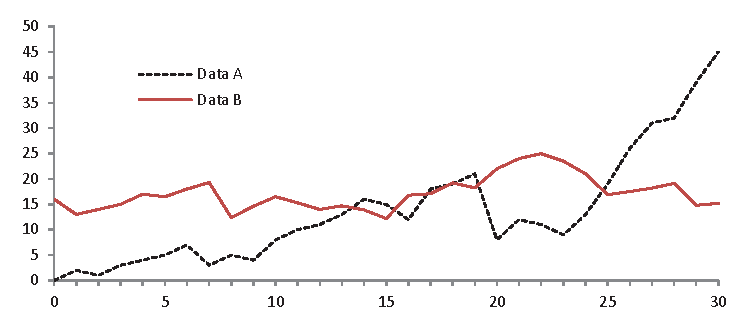
\includegraphics[width=\textwidth]{figures/fig1}
\caption{A figure caption is always placed below the illustration.
Please note that short captions are centered, while long ones are justified by the macro package automatically. The text within graphics should be readable in the printed version.} 
\label{fig:fig1}
\end{figure}

\begin{theorem}
This is a sample theorem. 
The run-in heading is set in bold, while the following text appears in italics. 
Definitions, lemmas, propositions, and corollaries are styled the same way.
\end{theorem}
%
% the environments 'definition', 'lemma', 'proposition', 'corollary',
% 'remark', and 'example' are defined in the LLNCS documentclass as well.
%
\begin{proof}
Proofs, examples, and remarks have the initial word in italics, while the following text appears in normal font.
\end{proof}
For citations of references, we prefer the use of square brackets and consecutive numbers. 
Citations using labels or the author/year convention are also acceptable. 
The following bibliography provides a sample reference list with entries for journal articles~\cite{Stol2016}, a book~\cite{Myers2012}, conference proceedings~\cite{Harrold1988}, and a web site~\cite{Schaffer2018}.

\subsection{Abbreviations}
\label{subsec:abbrev}

To use acronyms in the document, simple declare them in the main.tex file and use them later.
For example, you might want to define \acp{rq}, which will then be always abbreviated as \ac{rq} for singular or \acp{rq} for plural.

List are also really easy to create:

\begin{itemize}
  \item One entry in the list
  \item Another entry in the list
\end{itemize}

\begin{enumerate}
  \item The labels consists of sequential numbers.
  \item The numbers starts at 1 with every call to the enumerate environment.
\end{enumerate}

\subsection{Code Listings}
\label{subsec:code}

Listings can either be created inside the text or imported:\footnote{See \url{https://www.overleaf.com/learn/latex/Code_listing} for a complete example.}
\begin{lstlisting}[language=C,label={lst:lstlisting}]
int main(int argc, char* argv[]) {
  return 0;
}
\end{lstlisting}
\section{Related Works}

    The detection of near-duplicates in web applications has been explored through various approaches across multiple domains, including information retrieval, computer vision, and web testing. This section introduces earlier methods, recent research, and state-of-the-art techniques and presents the definitions of near-duplicates used in our work \cite{yandrapally_near-duplicate_2020}. 

    \subsection{Earlier Research}
     
        In the information retrieval domain, near-duplicate detection techniques primarily originate from search engines, where the focus is on the content of web pages. Due to the vast amount of data, performance often precedes accuracy. Hashing techniques, such as Simhash used by Google, have proven effective for this purpose \cite{charikar_similarity_2002}. These methods typically aim to identify near-duplicates between different sites rather than within the same site.
        
        To use another representation besides the \ac{dom} tree, some techniques from computer vision could be used, which employ screenshots of web pages. These techniques operate at various levels of granularity, utilizing techniques like colour histograms or image hashing. However, these techniques face challenges with responsive websites that alter their appearance based on device characteristics \cite{swain_indexing_1992,yang_block_2006}. 
        
        In web testing, near-duplicate detection methods have primarily focused on \ac{dom}-based abstractions. The \ac{rted} method leverages the \ac{dom} to calculate the minimum sequence of node edit operations required to transform one \ac{dom} tree into another \cite{pawlik_efficient_2015}. This method emphasizes structural similarities between web pages.
        
        Yandrapally et al. 2020 \cite{yandrapally_near-duplicate_2020} conclude that despite these efforts, no single method was sufficient for web testing, prompting the development of new approaches. Furthermore, they propose a finer-grained classification of cosmetic (irrelevant changes like different advertisements), dynamic data (data changes with the same page structure), and duplication (addition or removal of equivalent web elements) categories. Overall, they define near-duplicates as states that do not change the overall functionality of a web page, typically differing only by small cosmetic changes.

    \subsection{Recent Research}
    
        Corazza et al. 2021 \cite{corazza_web_2021} propose a new approach utilizing the \ac{dom} tree and tree kernel functions to compute similarities between tree structures. Tree kernel functions compute the similarity between tree structures, besides \ac{dom} trees they are also used on abstract syntax trees for clone detection. The authors employed a supervised ad hoc classifier on similarity vectors based on tree kernel functions. Despite their efforts, their approach showed only marginal improvements over older methods reviewed by Yandrapally et al. 2020 \cite{yandrapally_near-duplicate_2020}. Definitions of near-duplicates in the paper remained inconsistent, with terms like "minor changes", "noticeable differences", and "minimal, insignificant changes" being used interchangeably.
        
        With the prevalence of component-based software engineering in modern web development, particularly with frameworks like React \cite{noauthor_technology_nodate}, new methodologies have been developed \cite{vale_twenty-eight_2016,krznar_current_2016}. Yandrapally et al. 2023 \cite{yandrapally_fragment-based_2023} applied this concept by using the \ac{vips} algorithm \cite{cai_vips_2003} to segment web pages into components. The VIPS algorithm works with a top-down approach, combining visual and structural information to fit lines between blocks without visually crossing them, resulting in a tree of fragments. The tree structure is then analyzed using \ac{apted} \cite{pawlik_tree_2016} and colour histograms \cite{swain_indexing_1992}. This integrated approach leverages visual and structural information to classify pages based on rule-based criteria. Their rule-based classifier includes the fine-grained classes proposed by Yandrapally et al. 2020 \cite{yandrapally_near-duplicate_2020}.
        
        Furthermore, neural embeddings represent a cutting-edge approach. For instance, Stocco et al. 2023 \cite{stocco_neural_2023} applied the doc2vec model to embed \ac{dom} representations and compute cosine similarities between these embeddings. These similarity vectors were then classified using a fully connected neural network. This neural network requires training and, therefore, labelled training data, making it more effort to adopt. Recent work-in-progress efforts have utilized distilBERT embeddings and fine-tuning to achieve better results. Definitions of near-duplicates in this context varied between "states similar in functionality" and "concrete instances of the same logical state with minor changes".

    \subsection{Definitions}
    
        These varied definitions and methods highlight the complexity and interpretative nature of detecting near-duplicates in web applications. Our \ac{llm}-based approach aims to address these limitations by leveraging large language models' advanced language understanding capabilities. We adopt the definition used by Yandrapally et al. 2020 \cite{yandrapally_near-duplicate_2020} without the fine-grained subcategories and minor linguistic simplification:
        
        \begin{definition}[Near-Duplicate]
        A given state pair is considered a functional near-duplicate if the changes between the states do not alter the overall functionality of either state.
        \end{definition}
        
        \begin{definition}[Distinct]
        A given state pair is considered functionally distinct if there is any semantic or functional difference between the two pages.
        \end{definition}
        
        \begin{definition}[Clone]
        A given state pair is considered a functional clone if they have no semantic, functional, or perceptible differences.
        \end{definition}
        
        

    \subsection{Dataset}
    
        All presented approaches use the dataset created by Yandrapally et al. 2020 \cite{yandrapally_near-duplicate_2020}, which contains approximately 100,000 labelled state pairs from nine open-source web applications. By manually labelling a large, labour-intensive dataset, Yandrapally et al. 2020 \cite{yandrapally_near-duplicate_2020} made research in this area comparable and facilitated newer methods, making it a defacto standard. This dataset is a benchmark for evaluating the effectiveness of near-duplicate detection methods. 
\section{Approach}

    This section outlines our methodology for using \acp{llm} to classify web pages into distinct and near-duplicates. The following subsection introduces \acp{llm}, and our approach is explained in depth afterwards.

\subsection{Large Language Models}
    \label{sec:approach:sub:llm}

    \acp{llm} are artificial intelligence systems designed to understand and generate human-like text \cite{vaswani_attention_2017}. These models, such as GPT-4 and Llama 3, leverage deep learning techniques, especially transformer architecture and are trained on vast amounts of diverse data, enabling them to perform a wide range of language-related tasks with high proficiency \cite{touvron_llama_2023,openai_gpt-4_2024}. The evolution of LLMs represents a significant milestone in \ac{nlp}. Early models focused on specific language tasks, but with the upcoming transformer architectures, models have demonstrated remarkable capabilities in understanding and generating natural language. The transformer architecture, introduced by Vaswani et al. 2017 at Google \cite{vaswani_attention_2017}, is based on self-attention mechanisms that allow the model to weigh the importance of different words in a sentence, enabling it to capture long-range dependencies more effectively than previous architectures like \ac{rnn} and \ac{lstm}. This has significantly improved various \ac{nlp} tasks.
    
    \acp{llm} come in different sizes (number of weights), each offering a trade-off between capability and resource consumption. Bigger models tend to perform better due to their increased capacity to understand and generate complex text. However, they require substantial computational resources, making them less practical for deployment in resource-constrained environments. Conversely, smaller models are more efficient but may not achieve the same level of performance as their larger counterparts \cite{brown_language_2020}. An important consideration in utilizing \acp{llm} is prompt sensitivity. Open-source models often exhibit variability in their output quality based on how the input prompt is phrased \cite{sclar_quantifying_2024}. This sensitivity necessitates careful prompt engineering to ensure consistent and high-quality outputs. Commercial models like GPT-4 mitigate this issue by fine-tuning with reinforcement learning through human feedback \cite{openai_gpt-4_2024}. 
    
    In the context of this research, \acp{llm} are employed to understand and classify HTML documents by leveraging their advanced text-understanding capabilities. One of the critical strengths of \acp{llm} is their generalization capability, which allows them to perform well on various tasks even with limited specific training data. This is achieved through different learning modes, such as few-shot, one-shot, and zero-shot. Few-shot means that a few task demonstrations are provided to the model as conditioning at inference time. One-shot is comparable to few-shot but only using one demonstration, and zero-shot is instead of using any examples, the task is described in plain words. These modes enable the models to generalize from few examples or task descriptions alone, making them highly adaptable to new and diverse tasks \cite{brown_language_2020,touvron_llama_2023}.

\subsection{The Proposed Approach}
    \label{sec:approach:sub:proposed}

    \begin{figure}[htbp]
        \label{fig:gscan}
        \centering
        \includesvg{figures/GeminiScan}
        \caption{Approach: solid for inference, dashed for prompt engineering}
    \end{figure}

    Figure 1 gives an overview of our approach to efficiently classify web pages by leveraging the strengths of both small and large \acp{llm}. The approach consists of an inference loop for classification and a feedback loop for prompt optimization.

    \subsubsection{Inference Loop}
    \label{sec:approach:sub:proposed:sub:inference}

    The inference loop, illustrated by solid lines in Figure 1, is designed to efficiently classify web pages using a small \ac{llm}. This loop involves several key steps: First, we selected a small \ac{llm} for inference to benefit from speed and efficiency while maintaining sufficient capability for the task. Preliminary experiments indicated that while a larger \ac{llm} could solve the task more effectively, it would be more computationally expensive and slower in generating output. One challenge we encountered was that the entire HTML file often exceeds the maximum input length of the small \ac{llm}. To address this, we filter the HTML file to include only the body tag, excluding scripts. This approach, consistent with previous research by \cite{corazza_web_2021}, ensures that the relevant content is processed. We opted for this simple filtering to avoid introducing complex preprocessing steps that would become unnecessary as the context length of \acp{llm} rapidly evolves.
    
    The prompt, concatenated with the two filtered HTML files, is fed into the small-scale model, generating 20 tokens as output. Tokens are the smallest units of text the model processes, such as words or punctuation marks. This token threshold was determined through preliminary experiments to ensure the classification is never cut off. Although the model is instructed to generate a reasoning explanation after the classification output, we filter the generated tokens to extract the classification result. The model's reasoning helps debug by highlighting misunderstandings or interpretation issues within the prompt, which is valuable information for the feedback loop. We must filter the generated tokens because the \ac{llm} does not always output the classification as the first word. Preliminary experiments showed a loss in effectiveness when strictly requiring the classification to be the first word. We have chosen to focus on distinguishing distinct and near-duplicate states, as current methods can detect clones effectively \cite{yandrapally_near-duplicate_2020}. 
    
    Despite extensive prompt engineering, we reached a performance ceiling with an F1 score of 0.6. As mentioned in Section \ref{sec:approach:sub:llm}, open-source \acp{llm} suffer from prompt sensitivity, which made further improvements labour intensive. Additionally, defining the problem in depth beyond high-level definitions prevalent in current research proved to be highly complex.

    \subsubsection{Feedback Loop}
    \label{sec:approach:sub:proposed:sub:feedback}

    To improve the initial prompt without extensive manual intervention, we introduced a feedback loop inspired by the training methods of large \acp{llm} using human feedback \cite{ouyang_training_2022}. Instead of humans, we utilize a big-scale \ac{llm} to provide feedback and improve the prompt. This approach has been validated by others, demonstrating that \acp{llm} can effectively serve as prompt engineers \cite{zhou_large_2023}. After predicting the class for the compared states, incorrectly classified results and their F1 scores are sent as a batch to the larger \ac{llm}, along with visual renderings of the respective web pages. Adding visual rendering was motivated by increasing the overall information given to the big-scale \ac{llm}. The large \ac{llm} then adapts the prompt to enhance classification accuracy in subsequent iterations. Our automated feedback loop improves the prompt's effectiveness significantly, leveraging the large \ac{llm}'s capability to understand and refine prompts based on detailed feedback from the inference loop.
\section{Evaluation}
    
        This section evaluates the effectiveness and efficiency of our proposed approach for detecting near-duplicate web pages, comparing it to state-of-the-art techniques. 
    
    \subsection{Dataset}
        \label{sec:eval:sub:data}

        We utilized the annotated dataset by Yandrapally et al. 2020 \cite{yandrapally_near-duplicate_2020}, which comprises 97.5k state pairs from nine open-source web applications. This dataset allows direct comparison with other approaches, including those discussed in the related works section. The original annotations include distinct, clone, and near-duplicate classifications. We removed all clone instances as they can be reliably detected using existing methods. Due to computational resource constraints, we focused on two applications: Addressbook and PetClinic. These were chosen to represent different web technologies: Addressbook is PHP-based, while PetClinic uses a JavaScript framework. Table 1 provides an overview of the dataset used in this study.

        \begin{table}[h]
            \centering
            \label{table:data}
            \begin{tabular}{llllll}
                \hline
                Application & Technology                          & States & Pairs\protect\footnotemark & Distinct & Near-Duplicates \\ \hline
                Addressbook & PHP-based, Javascript               & 131    & 8515  & 6142     & 2347            \\
                PetClinic   & Angular (JavaScript), Spring (Java) & 149    & 11026 & 9411     & 1613            \\ \hline
                Total       &                                     & 280    & 19541 & 15553    & 3960               
            \end{tabular}
            \caption{Manual Classifications and Technology of Web Applications}
        \end{table}

        \footnotetext{28 Clones were emitted}

    \subsection{Implementation}
        \label{sec:eval:sub:impl}

        Our implementation utilizes two language models:

        \begin{itemize}
            \item Llama 3 8B \cite{touvron_llama_2023}, an open-source model chosen for greater control.
            \item GPT-4o \cite{noauthor_gpt-4o_nodate}, employed for the feedback loop due to resource constraints of hosting a big model ourselves.
        \end{itemize}
        
        We used the Python library BeautifulSoup for HTML preprocessing. The implementation was run on an Nvidia A100 GPU with 40GB RAM. The code for preprocessing and prediction is openly available for reproducibility \footnote{\url{https://github.com/H3nkl3r/GeminiScan}}.
    
    \subsection{Experimental Procedure}
        \label{sec:eval:sub:proc}
    
        The feedback loop was executed 12 times, with each iteration processing 100 state pairs. Resource limitations and the observed saturation of the F1 score determined this number. We used the F1 score as the primary metric for the feedback loop.
        \ac{llm} output was generated in batches of 8, the maximum batch size accommodated by the GPU's RAM. Furthermore, we used the recommended HuggingFace settings of $temperature=0.6$ and $top_p=0.9$.
        For performance evaluation, we employed precision, recall, and F1-score. These metrics were chosen for their effectiveness in measuring classification performance and to facilitate comparison with other approaches.
    
    \subsection{Baseline}
        \label{sec:eval:sub:base}
    
        We compared our approach to the following baselines:

        \begin{itemize}
            \item A naive baseline of always predicting "distinct", given the imbalanced nature of the dataset.
            \item \ac{rted} \cite{pawlik_efficient_2015}, previously identified as the fastest method before the introduction of FragGen and WebEmbed.
            \item WebEmbed by Stocco et al. 2023 \cite{stocco_neural_2023}
            \item FragGen by Yandrapally et al. 2023 \cite{yandrapally_fragment-based_2023}
        \end{itemize}

        WebEmbed and FragGen are strong benchmarks due to their superior performance in near-duplicate detection and usewelche von beiden?
11:47
 of the same evaluation data. Please note that FragGen does not report recall and precision.
        It should be noted that our approach uses binary classification (near-duplicate or distinct), while the baselines employ multi-class classification. However, we deemed this comparison valid due to the dataset's negligible number of clone instances (0.14\%).

    \subsection{Prompt}
        \label{sec:approach:sub:proposed:sub:prompt}

        A critical component of our approach is the prompt design for the \ac{llm}, which was iteratively refined through an automated feedback loop. This process produced a final prompt consisting of a system prompt and a user prompt.
        The system prompt (Listing \ref{lst:SysPrompt}) establishes the context and defines the task:
    
    \begin{lstlisting}[breaklines, caption={Final System Prompt},captionpos=b, label={lst:SysPrompt}]
    You are an intelligent agent skilled in natural language processing and web development. Your task is to classify pairs of HTML files into two categories: "near duplicate" or "distinct". "Near duplicate" HTML files represent the same logical state with minor differences. "Distinct" HTML files represent different logical states, particularly if they serve different purposes or contain significantly different content. For example, if one file is a group management page and the other is a shopping list page, they must be classified as "distinct". Such functional differences must lead to a "distinct" classification, even if the overall structure is similar.
    \end{lstlisting}
    The user prompt (Listing \ref{lst:UsrPrompt}) provides more detailed instructions:

    \begin{lstlisting}[breaklines, caption={Final User Prompt},captionpos=b, label={lst:UsrPrompt}]
    I will provide you with two HTML files. Please analyze them and determine whether they are "near duplicate" or "distinct". Provide a detailed explanation of your reasoning based on the structure, content, navigation elements, and any significant differences in elements and functionality. Pay special attention to functional differences such as different purposes, form actions, methods, and significant content differences. If there are any significant functional differences, such as different purposes (e.g., one page is for group management and the other is for displaying a shopping list) or significant content differences (e.g., one file has a form and the other has a table), classify the files as "distinct". HTML File 1: <html> HTML File 2: <html> Based on the analysis of the above HTML files, are they "near duplicate" or "distinct"? Please explain your reasoning. Consider factors such as structure, content, navigation elements, and any significant differences in elements and functionality. Highlight any functional differences, especially different purposes and significant content differences. If the pages serve different purposes or have significant content differences (e.g., one page is for group management and the other is for displaying a shopping list, or one file has a form and the other has a table), classify them as "distinct."
    \end{lstlisting}
        This prompt, generated through our feedback loop, demonstrates several key characteristics:
        \begin{itemize}
            \item Task Definition: It clearly defines the classification task and the categories ("near-duplicate" or "distinct").
            \item Reasoning Requirement: The prompt asks for detailed explanations, leveraging the \ac{llm}'s reasoning capabilities.
            \item Focus Areas: It highlights specific aspects, such as structure, content, navigation elements, and functionality.
            \item Examples: The prompt provides examples of distinct cases which may help guide the model's decision-making process.
            \item Repetition: Key points are reiterated, potentially reinforcing their importance to the \ac{llm}.
        \end{itemize}

        Notably, the prompt does not provide specific examples for near-duplicate cases. 
        The automated nature of the prompt generation demonstrates the effectiveness of our feedback loop in refining the prompt without manual intervention. This approach allowed us to overcome the initial performance ceiling and prompt sensitivity issues often associated with open-source \acp{llm}.
    
    \subsection{Results}
        \label{sec:eval:sub:result}

        Table 2 presents the macro-averaged F1 scores, precision, and recall for our approach (GeminiScan) alongside the baseline methods.

        \begin{table}[htbp]
            \centering
            \label{table:f1}
            \begin{tabular}{lcccccc}
                \hline
                & \multicolumn{3}{c}{Addressbook} & \multicolumn{3}{c}{PetClinic} \\ \cline{2-4} \cline{5-7}
                Method              & $F_1$ Score   & Precision     & Recall        & $F_1$ Score   & Precision     & Recall        \\ \hline
                Distinct            & 0.42          & 0.86          & 0.5           & 0.46          & 0.93          & 0.5           \\
                RTED                & 0.70          & 0.69          & 0.73          & 0.73          & 0.70          & 0.77          \\
                WebEmbed            & \textbf{0.92} & \textbf{0.89} & \textbf{0.95} & 0.81          & \textbf{0.77} & 0.85          \\
                FragGen             & 0.89          & -             & -             & \textbf{1.00} & -             & -             \\
                \textit{GeminiScan} & 0.87          & 0.85          & 0.92          & 0.78          & 0.74          & \textbf{0.90} \\ \hline
            \end{tabular}
            \caption{Macro-averaged $F_1$ scores for Addressbook and PetClinic}
        \end{table}

        Our approach outperforms \ac{rted} by 24\% and 7\% on Addressbook and PetClinic, respectively. It achieves comparable performance to state-of-the-art methods, with F1 scores 5\% and 2\% lower than WebEmbed for Addressbook and PetClinic and 4\% and 22\% lower than FragGen. GeminiScan shows good values for recall, being the 3\% lower as WebEmbed on Addressbook and 6\% better on PetClinic.
        Figures \ref{fig:conv_address} and \ref{fig:conf_pet} show the confusion matrices for Addressbook and PetClinic classifications.

        \begin{figure}[ht]
          \centering
          \begin{subfigure}[b]{0.48\textwidth}
            \includesvg[width=\textwidth]{figures/confusion_matrix_address.svg}
            \caption{Confusion Matrix of Addressbook classification task}
            \label{fig:conv_address}
          \end{subfigure}
          \hfill
          \begin{subfigure}[b]{0.48\textwidth}
            \includesvg[width=\textwidth]{figures/confusion_matrix_petclinic.svg}
            \caption{Confusion Matrix of PetClinic classification task}
            \label{fig:conf_pet}
          \end{subfigure}
          \caption{Confusion matrices for classification tasks}
          \label{fig:both_matrices}
        \end{figure}

        In the Addressbook classification task (Figure \ref{fig:conv_address}), the model correctly identifies 5165 distinct pages and misclassifies 977 distinct pages as near-duplicates. Additionally, the model correctly identifies 2345 near-duplicates but misclassifies two near-duplicates as distinct pages. For the PetClinic classification task (Figure \ref{fig:conf_pet}), the model correctly classifies 7827 distinct pages and incorrectly labels 1584 distinct pages as near-duplicates. It accurately identifies 1559 near-duplicates while misclassifying 54 near-duplicates as distinct pages.

        Overall, the model demonstrates strong performance in identifying distinct pages and effectively detecting near-duplicates. However, there is a notable number of false negatives, where distinct pages are misclassified as near-duplicates. Conversely, the model rarely misclassifies near-duplicates as distinct. Regarding efficiency, our approach averages 455ms per classification for Addressbook and 350ms for PetClinic on an Nvidia A100 GPU with a batch size of 8. Classification time varies with the size of the \ac{dom} tree, which affects the prompt length. The progression of the F1 score through the feedback loop was high initially. Including form actions and examples, the feedback loop improved the F1 score by 0.2 for each. Afterwards, the progression got smaller and eventually saturated.

        
\section{Discussion}

    Our approach to near-duplicate web page classification using Large Language Models (LLMs) demonstrates promising performance, albeit not surpassing current state-of-the-art methods. However, our method offers significant benefits and potential for future improvements.
    
    \subsection{Strengths and Applicability}
        A key strength of our approach lies in its generalizability. The model's classification is solely based on input data without relying on pre-trained, application-specific features. This characteristic enhances the method's applicability across diverse web applications. While we used page pairs from the same dataset for prompt improvement, the resulting prompt remains general and not specific to the applications used in this study.
        Unlike other approaches that require extensive labelled training data, our method can be applied directly without preliminary data labelling. This significantly lowers the entry barrier for users, albeit at the cost of slightly lower precision and recall compared to specialized, data-intensive methods.
        
    \subsection{Interpretability and Explainability}
        One notable advantage of using \acp{llm} is the human-readable output, which enhances interpretability and explainability. The model provides reasoning for its decisions, allowing for better understanding and potential improvements in task description.
        Notably, this reasoning has revealed that current definitions in research are often too simplistic. The \ac{llm} identifies numerous ways to argue for alternative classifications, highlighting the considerable interpretative range within existing definitions. This insight underscores the need for more nuanced and comprehensive definitions in near-duplicate detection research. Still, the underlying mechanism of \acp{llm} on calculating the output remains a black box.
        
    \subsection{Performance Analysis}
        Our model successfully identifies distinct pages and accurately detects near-duplicates. This capability is crucial for creating comprehensive and efficient test suites, avoiding redundant test cases while ensuring coverage of unique scenarios.
        However, we observed many false negatives where distinct pages were misclassified as near-duplicates. This tendency to err on the side of caution by flagging more pages as potential near-duplicates presents a double-edged sword:
        \begin{itemize}
        \item It helps avoid duplicate tests, saving time and resources.
        \item It risks missing unique cases that should be tested separately, potentially compromising test suite completeness.
        \end{itemize}
        Notably, the model rarely misclassifies near-duplicates as distinct, which is beneficial for maintaining an efficient test suite without unnecessary redundancy. We have looked at the wrongly classified examples and often concluded that these are hard-to-decide edge cases, for instance, an address book with zero entries vs ten entries.
        
    \subsection{Open Challenges}
        Several open challenges in our study present opportunities for future research:
        \begin{itemize}
            \item \textbf{Resource Constraints:} Due to limited resources, we could not further optimize the prompt through additional feedback loop iterations. Extended resources could allow for more iterations and exploration of different optimization paths. Moreover, resource usage is an overall challenge as \acp{llm} requires much more resources than other approaches.
            
            \item \textbf{Dataset Characteristics:} The dataset used may not fully represent real-world scenarios. It was created offline, potentially missing the dynamic exploration patterns of a live crawler. Additionally, the dataset's imbalance might not reflect all web applications, where near-duplicates could outnumber distinct pages.
            
            \item \textbf{HTML Preprocessing:} Our approach of trimming HTML to exclude script tags may have contributed to the poorer performance on JavaScript-based applications like PetClinic. Future work could explore more sophisticated preprocessing techniques or increased context sizes to include complete \ac{dom} structures.
            
            \item \textbf{Prompt Design:} The feedback loop did not include examples of near-duplicates in the prompt, potentially influencing the model's behaviour. Further research could investigate the impact of balanced example inclusion. In our experiments, the \ac{llm} clearly showed an understanding of the HTML, and the prompt determined the goodness of the results. Therefore, further prompt or feedback loop improvements could yield better results.

            \item \textbf{Probabilistic Approach:} All probabilistic machine learning techniques must address the issue that outcomes may not always match expectations because there is no well-defined deterministic rule governing the classification process. According to more recent studies, the term hallucinations may be masking the real issue, which is that \acp{llm} produces what seems most human rather than the truth. They conclude that "bullshitting" would be a more appropriate term to use in place of hallucinations \cite{hicks_chatgpt_2024}. 
        \end{itemize}
        
    \subsection{Future Directions}
        The rapid advancements in \ac{llm} technology present exciting opportunities for improving our approach:
        \begin{itemize}
            \item \textbf{Evolving \ac{llm} Capabilities:} As language and code understanding in \acp{llm} improve, along with increased efficiency, our approach may become more suitable for production use. Growing context sizes in \acp{llm} could enable the processing of entire \ac{dom} structures without trimming, potentially improving accuracy. This could also facilitate one-shot or few-shot approaches with provided examples.
            
            \item \textbf{Multi-modal Approaches:} While hallucination issues hindered our initial experiments with vision learning models, the coming release of multi-modal models like Llama could offer new avenues for exploration.

            \item \textbf{Synergies:} Duplicate or near-duplicate detection is not a problem only observed in web testing. Thus, exploring further synergies with other areas like process mining could also add value. 
        \end{itemize}

\section{Conclusion}
    \label{sec:conclusion}
    
    This paper introduced GeminiScan, a novel LLM-based approach to near-duplicate detection in web testing. By combining a small-scale LLM for efficient inference with a large-scale LLM for prompt optimization, our method addresses challenges in semantic understanding and generalization.
    
    Evaluation of the Addressbook and PetClinic applications from the Yandrapally et al. 2020 dataset demonstrated competitive performance, with F1 scores of 0.87 and 0.78, respectively. Furthermore, GeminiScan outperforms traditional methods like RTED and approaches the effectiveness of state-of-the-art techniques such as WebEmbed and FragGen. Key strengths include strong performance in identifying distinct pages, effective near-duplicate detection, and a low false positive rate. While computational requirements present a challenge, our automated feedback loop for prompt optimization showcases the potential for continuous improvement. Future work could focus on expanding the evaluation to more diverse web applications, reducing computational requirements, and further improving classification accuracy.
    
    GeminiScan represents a significant step in applying advanced \ac{nlp} techniques to web testing, opening new opportunities for research in software quality assurance. As LLM technology rapidly advances, we anticipate further improvements in the efficiency and effectiveness of near-duplicate detection in web testing. This could possibly lead to the replacement of manual test creation in the future.
%
% ---- Appendix ----
%
%\appendix
%\section{Appendix}
\label{sec:appendix}

Anything additional goes here \dots
%
% ---- Bibliography ----
%
\bibliographystyle{splncs04}
\bibliography{library.bib}
%
\end{document}
